\chapter{Antecedentes}

\section{Control de flujo de información}
Los lenguajes con tipado de seguridad para el control del flujo de la información clasifican los valores de un programa con respecto a sus niveles de confidencialidad, expresado mediante una \textit{lattice}\footnote{Un orden parcial, donde todo par de elementos tiene un único supremo e ínfimo} de etiquetas de seguridad. Por ejemplo, con la \textit{lattice} de dos niveles de seguridad \texttt{L} $\sqsubseteq$ \texttt{H} se puede distinguir entre valores públicos o de baja confidencialidad (\texttt{L}) y valores privados o de alta confidencialidad (\texttt{H}). Un sistema de tipos con control de flujo asegura de forma estática el cumplimiento de la propiedad \emph{noninterference}~\cite{noninterference}, esto es, que la información confidencial no fluya directa o indirectamente hacia canales públicos~\cite{volpanoAl:S96}.

En el siguiente ejemplo se muestra un código anotado con niveles de seguridad:

\begin{ej} \ \\
  \normalfont
  \label{ej2-1}
\begin{lstlisting}
  String@L login(String@L guess, String@H password) {
    if (password == guess) return "Login successful";
    else return "Login failed";
  }
\end{lstlisting}
\end{ej}

Se dice que ocurrió un \emph{flujo implícito} cuando un programa da conocimiento de una variable de baja confidencialidad, en un contexto de alta confidencialidad. En el ejemplo \ref{ej2-1}, se da conocimiento de un literal (que por convención es considerado de baja confidencialidad) en un contexto determinado por la operación de comparación en la condición del \texttt{if}, la cual retorna un valor de alta confidencialidad.

Para detectar un flujo implícito, se utiliza el concepto de \textit{program counter} (PC) para seguridad~\cite{pc}, el cual permite considerar el contexto de ejecución de una instrucción en las reglas del sistema de tipos. En el ejemplo \ref{ej2-1}, las instrucciones de retorno se ejecutan con un PC igual al nivel de seguridad de retorno de la condición.

A pesar de que noninterference es una propiedad atractiva para la especificación de sistemas seguros, se considera muy estricta en la práctica, debido a que previene que la información confidencial tenga cualquier tipo de influencia en una salida observable de un programa. En efecto, el programa de \texttt{login} del ejemplo \ref{ej2-1} rompe con la propiedad, debido a que un observador público puede aprender acerca de la variable confidencial \texttt{password} observando la salida del programa para distintas ejecuciones.

Sin embargo, deseamos que el programa de \texttt{login} sea aceptado, pues de otra forma no tendríamos cómo realizar la autenticación. Para solucionar este problema, los lenguajes de seguridad adicionan mecanismos para disminuir el nivel de seguridad de un valor confidencial, implementados de diferentes formas~\cite{sabelfeldSands:JCS09}. Una de ellas, por ejemplo en Jif~\cite{jif} es usar un operador \texttt{declassify}, como se indica en el siguiente ejemplo, \emph{desclasificando} la comparación de igualdad del parámetro confidencial \texttt{password} con el parámetro público \texttt{guess}

\begin{lstlisting}
  String@L login(String@L guess, String@H password) {
    if (declassify(password == guess)) return "Login Successful";
    else return "Login failed";
  }
\end{lstlisting}

Esto no corresponde a una amenaza de seguridad, debido a que el resultado de la operación de comparación es negligible con respecto al parámetro privado \texttt{password}. Sin embargo, usos arbitrarios del operador \texttt{declassify} pueden resultar en serias fugas de información; por ejemplo, \texttt{declassify(password)} da conocimiento absoluto sobre el valor de la variable.

Varios mecanismos se han explorado para controlar el uso de desclasificación, y poder asegurar además una propiedad de seguridad para el programa~\cite{sabelfeldSands:JCS09}. En esta dirección, Cruz et al.~\cite{cruzAl:ecoop2017} recientemente propusieron \textit{type-based declassification} como un mecanismo de desclasificación que conecta la abstracción de tipos con una forma controlada de desclasificación, en una manera intuitiva y expresiva, proveyendo garantías formales sobre la seguridad del programa.

En \textit{type-based declassification} los tipos tienen dos facetas; la faceta privada, que refleja el tipo de implementación, y la faceta pública, que refleja las operaciones de desclasificación sobre los valores de dicho tipo. Por ejemplo, el tipo $\mathtt{StringEq} \triangleq [\mathtt{eq} : \mathtt{String} \rightarrow \mathtt{Bool}]$ autoriza la operación \texttt{eq} sobre un String. Entonces se puede usar el tipo de dos facetas $\mathtt{String} < \mathtt{StringEq}$, en donde String es un subtipo de StringEq, para controlar la operación de desclasificación de la igualdad sobre \texttt{password}.

\begin{lstlisting}
  String<String login(String<StringEq password, String<String guess) {
  	if (password.eq(guess)) return "Login successful";
  	else return "Login failed";
  }
\end{lstlisting}

Al igual que en tipado de seguridad con etiquetas (\texttt{L} y \texttt{H}), la faceta de desclasificación es parte de la jerarquía de tipos, la que forma una lattice como se muestra en la figura \ref{latticeTBD}. Si la faceta pública coincide con la faceta privada, entonces toda operación sobre el valor estará autorizada. Cuando esto sucede, se refiere usualmente a la faceta pública con \texttt{Bot}, por encontrarse siempre en la parte inferior de la lattice.

	\begin{figure}[ht]
		\centering
		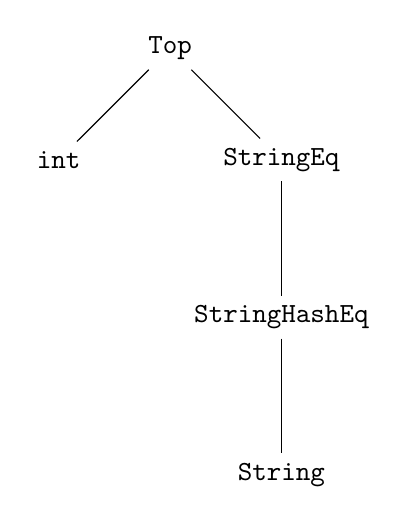
\begin{tikzpicture}[node distance=2cm]
			\node(Top) 												{\texttt{Top}};
			\node(StringEq)		[below right of=Top]			{\texttt{StringEq}};
			\node(StringHashEq)      [below of=StringEq]       {\texttt{StringHashEq}};
			\node(String)				[below of=StringHashEq]       {\texttt{String}};
			\node(int)					[below left of=Top] 			{\texttt{int}};
			\draw(Top)      -- (StringEq);
			\draw(Top)      -- (int);
			\draw(StringEq)      -- (StringHashEq);
			\draw(StringHashEq)      -- (String);
		\end{tikzpicture}
    \label{latticeTBD}
		\caption{lattice de tipos de dos facetas}
	\end{figure}

Cuando se quiere referir a una faceta pública vacía o que no autoriza ninguna operación, se usa \texttt{Top}, por encontrarse en la parte superior de la lattice.

En estricto rigor, los métodos declarados en la faceta pública también poseen tipos de dos facetas en sus firmas. Así, el tipo StringEq visto anteriormente se define como $\mathtt{StringEq} \triangleq [\mathtt{eq} : \mathtt{String<String} \rightarrow \mathtt{Bool<Bool}]$.

Existen dos reglas principales para comprobar que un programa con facetas de desclasificación se encuentra bien tipado. En primer lugar, la llamada a un método sobre un valor cuya faceta pública autoriza la operación, retorna la faceta pública que haya sido declarada como retorno para aquella operación. Por ejemplo, si tenemos un valor con faceta pública $\mathtt{StringHashEq} \triangleq [\mathtt{hash} : \mathtt{String<String} \rightarrow \mathtt{String<StringEq}]$, y llamamos al método $\mathtt{hash}$ sobre este valor, la faceta de retorno de esa llamada será $\mathtt{String<StringEq}$. A esta regla se le llama \texttt{TmD}.

La segunda regla expresa que la llamada a un método sobre un valor cuya faceta pública no autoriza la operación, retorna \texttt{Top}. Esto ocurre, por ejemplo, si llamamos al método $\mathtt{hash}$ sobre un valor que declara la faceta pública $\mathtt{StringEq}$. A esta regla se le llama \texttt{TmH}.

La propiedad de seguridad que se demuestra para el sistema de tipos de \textit{type-based declassification} es una forma de noninterference con políticas de desclasificación, denominada \textit{Relaxed noninterference}. Un lenguaje de seguridad que cumple esta propiedad, garantiza que la información confidencial sólo puede fluir hacia canales públicos de forma controlada, por medio de las políticas de desclasificación.

\section{Inferencia de tipos}
\subsection{Objetivo y usos}
La inferencia de tipos es el proceso de determinar los tipos para las expresiones de un programa, basado en cómo son usadas. Tener un mecanismo de inferencia en un lenguaje de programación puede ser muy útil, debido a que da la posibilidad al programador de omitir las declaraciones de tipo para algunos identificadores. Consideremos el siguiente ejemplo:

\begin{lstlisting}
  int foo(int a, int b) {
    int c = a + b;
    return c;
  }
\end{lstlisting}

Supongamos que la suma solo está definida para números. Aquí, se considera redundante declarar el tipo de la variable \texttt{c}, debido a que la suma de dos números enteros siempre da como resultado un número entero. De la misma forma, podría ser considerado redundante declarar los tipos de los parámetros \texttt{a} y \texttt{b}, debido a que son utilizados como sumando en la asignación a la variable \texttt{c}, que fue declarada como \texttt{int}.

\subsection{Variables de tipo} \label{schemes}
Los lenguajes de programación que tienen un mecanismo de inferencia de tipos, pueden expresar sus tipos mediante \textit{type schemes}, los cuales incluyen variables de tipo y tipos concretos. Una variable de tipo es un tipo que no ha sido determinado.

Consideremos el mismo ejemplo, pero ahora omitiendo la declaración del tipo de la variable \texttt{c}.

\begin{lstlisting}
  int foo(int a, int b) {
    var c = a + b;
    return c;
  }
\end{lstlisting}

Para tipar la variable \texttt{c}, el sistema de tipos le asignará una variable de tipo $\alpha$, y generará \textit{side conditions} al aplicar las reglas del sistema de tipos. En este caso, la \textit{side condition} dice que el tipo de \texttt{c}, es decir, $\alpha$, tiene que ser igual al tipo del lado derecho de la asignación, es decir, \texttt{int}.

\subsection{Constraints} \label{constraints}
En el ejemplo anterior, se expresó la \textit{side condition} con lenguaje natural. Como el objetivo es automatizar el proceso de inferencia, se utilizan constraints para expresar las \textit{side conditions} generadas por la aplicación de una regla del sistema de tipos.

Las constraints sirven para expresar una relación entre dos tipos. Esta relación puede ser de igualdad o de subtyping. En el ejemplo anterior, la \textit{side condition} puede ser representada mediante la constraint $\{\alpha = int\}$.

El uso de constraints permite la presentación de un algoritmo de inferencia de forma modular, como un generador de constraints y un solucionador de constraints. En el siguiente ejemplo, se supone que \texttt{num} es heredado por otros tipos numéricos.

\begin{lstlisting}
  foo(int a, float b, bool cond) {
    var c;
    if (cond) c = a;
    else c = b;
    return c;
  }
\end{lstlisting}

El sistema de tipos asignará los siguientes tipos al programa:
\begin{lstlisting}[mathescape=true]
  $\alpha$ foo(int a, float b, bool cond) {
    $\beta$ c;
    if (cond) c = a;
    else c = b;
    return c;
  }
\end{lstlisting}
Y generará el set de constraints de subtyping $C: \{\beta <: \alpha, int <: \beta, float <: \beta\}$, de donde se deben resolver los tipos de las dos variables de tipo generadas. Notemos que $\beta$ debe ser supertipo de \texttt{int} y \texttt{float}. El mejor tipo que cumple con ambas constraints es \texttt{num}.
\subsection{Unificación}
La unificación es el proceso de encontrar una substitución que hace iguales a dos términos. Aplicado a un set de constraints, se genera un mapeo de variables de tipo a tipos concretos, que satisfacen cada una de las constraints.

Si las constraints son de igualdad, la unificación consiste en realizar substituciones sucesivas hasta resolver cada uno de los tipos. En cambio, si las constraints son de subtyping, se deben realizar las operaciones \texttt{meet} (el ínfimo entre dos elementos, $a \wedge b$) y \texttt{join} (el supremo entre dos elementos, $a \vee b$) sobre la lattice que conforma la jerarquía de tipos, cuando sea pertinente.

Por ejemplo, en el set de constraints generado en el ejemplo anterior, para resolver el tipo de $\beta$ se debe realizar la operación \texttt{join} entre \texttt{int} y \texttt{float}, lo que da como resultado \texttt{num}. Luego, el set de constraints se reduce a $C: \{\beta <: \alpha, num <: \beta\}$, donde ahora se puede substituir $\beta$ por \texttt{num}, lo que genera finalmente el mapeo $S: \{\beta \rightarrow num, \alpha \rightarrow num\}$.
\subsection{Inferencia de tipos de seguridad}
Como se vio en la sección \ref{sectype}, los tipos de seguridad conforman una lattice con relaciones de subtyping, al igual que la jerarquía de tipos. En consecuencia, es posible formular un algoritmo de inferencia basado en constraints para tipos de seguridad.

En esta dirección, Pottier \textit{et al.}~\cite{Pottier} estudiaron un análisis de control de flujo basado en tipos para un lenguaje con referencias, excepciones y polimorfismo, con un sistema de tipos basado en constraints e inferencia de tipos decidible.
